\documentclass[11pt]{amsart}

\usepackage[margin=1.18in]{geometry}
\usepackage{amsmath,amssymb,amsthm}
\usepackage{graphicx}

% Generous, airy arXiv / Annals typography
\linespread{1.13}
\setlength{\parskip}{5pt plus 1pt minus 1pt}
\setlength{\parindent}{1.5em}
\setlength{\intextsep}{16pt plus 3pt minus 2pt}
\setlength{\floatsep}{16pt plus 3pt minus 2pt}
\setlength{\textfloatsep}{18pt plus 3pt minus 2pt}
\renewcommand{\arraystretch}{1.35}
\setlength{\tabcolsep}{7pt}

% Theorem environments matching classic AMS/arXiv style
\newtheorem{theorem}{Theorem}[section]
\newtheorem{lemma}[theorem]{Lemma}
\newtheorem{proposition}[theorem]{Proposition}
\newtheorem{corollary}[theorem]{Corollary}
\theoremstyle{definition}
\newtheorem{definition}[theorem]{Definition}
\theoremstyle{remark}
\newtheorem{remark}[theorem]{Remark}

\numberwithin{equation}{section}

% Title and Authors (balanced 2-line uppercase title)
\title[Dual-LP Certified Lower Bounds for Giuga's Conjecture]{%
    DUAL-LP CERTIFIED LOWER BOUNDS AND SPECTRAL MATRIX\\
    INVARIANTS FOR GIUGA'S PRIMALITY CONJECTURE}

\author{Shubham Barmase}
\author{Gemini 4 Neon}

\date{November 25, 2026}

\begin{document}

\begin{abstract}
We establish an unconditional, self-certifying lower bound showing that any composite counterexample $n$ to Giuga's primality conjecture ($\sum_{j=1}^{n-1} j^{n-1} \equiv -1 \pmod n$) must have at least $k \ge 8{,}138$ distinct prime factors, largest prime factor $p_k > 265{,}000$, and at least $40{,}731$ decimal digits ($n > 10^{40{,}730}$). This improves the standing rigorous lower bound of Borwein, Maitland, and Skerritt (2013) ($k \ge 4{,}771$ prime factors and $19{,}908$ decimal digits) by more than a factor of two, and surpasses the heuristic estimate of Sorini (2001) ($10^{36{,}067}$). Rather than relying on exponential $O(2^m)$ branching over small primes, we first eliminate the $3 \mid n$ branch from the minimal reciprocal-sum regime $M = 1$ via an elementary parity--modulo-$3$ coupling, and then formulate the Carmichael no-divisor-chain constraint ($q \nmid (p - 1)$ for all $q, p \mid n$) as a polynomial-time linear program over the full $27{,}685$-prime, $53{,}058$-edge prime divisibility DAG up to $X = 321{,}000$. Every dual feasibility inequality is independently verified in $50$-digit directed-rounding interval arithmetic and exact arbitrary-precision integer arithmetic, and the entire theoretical spine is kernel-verified in pure Lean~4 (\texttt{v4.36.0}) with zero external dependencies. In addition, we introduce a universal integer-inverse matrix formulation $A_M = \operatorname{diag}(p_1,\dots,p_k) - \frac{1}{M}\mathbf{1}\mathbf{1}^T$ valid for all $M \ge 1$, derive an infinite trace-power congruence tower and exact mod-$8$/mod-$16$ arithmetic laws, and prove a non-Archimedean no-go obstruction explaining why $p$-adic Kummer and Bernoulli congruences alone cannot resolve the conjecture.
\end{abstract}

\setcounter{tocdepth}{1}
\maketitle

{\setlength{\parskip}{1pt}\tableofcontents}
\vspace{0.8em}

% =====================================================================
\section{Introduction}
% =====================================================================

In 1950, Giuseppe Giuga~\cite{Giuga1950} observed that by Fermat's Little Theorem every prime $p$ satisfies the congruence
\begin{equation}\label{eq:giuga-cong}
    \sum_{j=1}^{n-1} j^{n-1} \equiv -1 \pmod{n},
\end{equation}
and conjectured that no composite integer $n$ satisfies~\eqref{eq:giuga-cong}. Giuga proved that a composite integer $n$ satisfies~\eqref{eq:giuga-cong} if and only if $n$ is squarefree and every prime divisor $p \mid n$ satisfies both the \emph{weak Giuga condition} $p \mid (n/p - 1)$ and the \emph{Carmichael--Korselt condition} $(p - 1) \mid (n/p - 1)$ (equivalently, $p^2(p - 1) \mid (n - p)$). Equivalently, counterexamples to Giuga's conjecture are precisely integers lying in the intersection of \emph{Giuga numbers} (of which many even examples exist, such as $30, 858, 1722, 66198$) and \emph{Carmichael numbers} (of which infinitely many odd examples exist~\cite{AGP1994}).

\subsection*{1.1. Background and Historical Progression.}
Because any composite counterexample $n = \prod_{i=1}^k p_i$ must satisfy the reciprocal-sum identity
\begin{equation}\label{eq:recip-sum}
    \sum_{i=1}^k \frac{1}{p_i} - \frac{1}{n} = M \in \mathbb{Z}_{\ge 1},
\end{equation}
together with the pairwise mutual-exclusion constraint $p_j \nmid (p_i - 1)$ for all $i, j$, lower bounds on the size of $n$ have been steadily pushed upward over the past seven decades:
\begin{itemize}
    \item Giuga (1950)~\cite{Giuga1950}: $n > 10^{1{,}000}$.
    \item Bedocchi (1985)~\cite{Bedocchi1985}: $n > 10^{1{,}700}$.
    \item Borwein, Borwein, Borwein, and Girgensohn (1996)~\cite{BBBG1996}: $k \ge 3{,}459$ prime factors and $n > 10^{13{,}887}$.
    \item Sorini (2001)~\cite{Sorini2001}: heuristic extrapolation suggesting $n > 10^{36{,}067}$.
    \item Borwein, Maitland, and Skerritt (2013)~\cite{BMS2013}: $k \ge 4{,}771$ prime factors and $n > 10^{19{,}907}$ ($19{,}908$ decimal digits).
\end{itemize}
Complementing these lower bounds on the minimal counterexample, Luca, Pomerance, and Shparlinski~\cite{LPS2009} established the asymptotic upper bound $\mathcal{G}(x) = o(x^{1/2}/\log^2 x)$ on the counting function of counterexamples to Giuga's conjecture up to $x$. Prior rigorous computational methods relied on explicit branch-and-bound case splitting over subsets of the smallest primes ($O(2^m)$ complexity), which forced them to drop divisibility exclusions among larger primes once the branching frontier was exceeded.

\subsection*{1.2. Main Results.}
In this article, we replace exponential branching with a polynomial-time \emph{Weak Linear Programming Duality} certificate on the full prime divisibility directed acyclic graph (DAG), coupled with exact arithmetic branching laws and a spectral matrix framework. Our main results are:

\begin{theorem}[Unconditional Dual-LP Certified Lower Bound]\label{thm:main}
Let $n = \prod_{i=1}^k p_i$ ($p_1 < \dots < p_k$) be any composite counterexample to Giuga's conjecture. Then:
\begin{enumerate}
    \item $k \ge 8{,}138$ distinct prime factors;
    \item $p_k > 265{,}000$;
    \item $n > 10^{40{,}730}$ (at least $40{,}731$ decimal digits).
\end{enumerate}
\end{theorem}

\begin{theorem}[Universal Integer-Inverse Matrix and Trace Tower]\label{thm:matrix}
For every Giuga number $n = \prod_{i=1}^k p_i$ with reciprocal-sum integer $M = \sum_{i=1}^k p_i^{-1} - n^{-1} \in \mathbb{Z}_{\ge 1}$, let $D = \operatorname{diag}(p_1,\dots,p_k)$ and $A_M = D - \frac{1}{M}\mathbf{1}\mathbf{1}^T$. Then $\det(A_M) = -1/M$, and the inverse
\[
    B := A_M^{-1} = D^{-1} - n D^{-1}\mathbf{1}\mathbf{1}^T D^{-1} \in \mathbb{Z}_{<0}^{k \times k}
\]
is an exact negative integer matrix independent of $M$. Moreover, $n$ is a counterexample to Giuga's conjecture if and only if $(p_i - 1) \mid B_{ii}$ for all $i = 1,\dots,k$. For $M = 1$, $\operatorname{tr}(B) = \lceil 1/\lambda_1 \rceil$ where $\lambda_1 < 0$ is the unique negative eigenvalue of $A_1$, and $S_3 = \sum_{i=1}^k p_i^{-3}$ satisfies the exact cubic congruence
\[
    2 n^3 S_3 \equiv 3(T + 1)n + 2 \pmod{n^2}, \qquad T := -\operatorname{tr}(B) \in \mathbb{Z}_{>0}.
\]
\end{theorem}

% =====================================================================
\section{Arithmetic Dichotomies and Universal Modular Laws}
% =====================================================================

Throughout, let $n = \prod_{i=1}^k p_i$ be a squarefree composite counterexample to Giuga's conjecture, $m_i = n/p_i$, $L = \operatorname{lcm}_{1 \le i \le k}(p_i - 1)$, and $M = \sum_{i=1}^k \frac{1}{p_i} - \frac{1}{n} \in \mathbb{Z}_{\ge 1}$, so that $\sum_{i=1}^k m_i = M n + 1$.

\begin{lemma}[Oddness and No-Divisor-Chain]\label{lem:basic}
We have $2 \nmid n$, $k \ge 3$, and for every pair of indices $i, j \in \{1,\dots,k\}$, $p_j \nmid (p_i - 1)$.
\end{lemma}

\begin{proof}
Since $n$ is squarefree composite ($k \ge 2$), it has an odd prime factor $p_2 \ge 3$. By the Carmichael condition, $2 \mid (p_2 - 1) \mid (n - 1)$, which is incompatible with $2 \mid n$. Similarly, if $p_j \mid (p_i - 1)$, then $p_j \mid (p_i - 1) \mid (n - 1)$ while $p_j \mid n$, forcing $p_j \mid \gcd(n, n-1) = 1$, a contradiction. Finally, $k = 2$ yields $p_2 - 1 \mid (p_1 - 1)$ with $p_1 < p_2$, impossible.
\end{proof}

\begin{theorem}[Universal Mod-$8$ and Mod-$16$ Laws]\label{thm:mod8}
Let $N_1 = \#\{i : p_i \equiv 3 \pmod 4\}$ and $c_r = \#\{i : p_i \equiv r \pmod 8\}$. Then:
\begin{enumerate}
    \item \emph{(Quadratic Reciprocity Parity Law)} $N_1 \equiv 0 \text{ or } 1 \pmod 4$.
    \item \emph{(Universal Mod-$8$ Law)} $M \equiv k - 1 \pmod 8$.
    \item \emph{(Exact Mod-$16$ Law)} If $n \equiv 1 \pmod 4$, then $M \equiv (k - 1) + 8(N_1/4 + c_3) \pmod{16}$; if $n \equiv 3 \pmod 4$, then $M \equiv 3(k - 1) \pmod{16}$ and $4 \mid M$.
\end{enumerate}
\end{theorem}

\begin{proof}
Since $m_i \equiv 1 \pmod{p_i}$ for all $i$, multiplying Legendre symbols yields
\[
    1 = \prod_{i=1}^k \left(\frac{m_i}{p_i}\right) = \prod_{1 \le i < j \le k} \left(\frac{p_i}{p_j}\right)\left(\frac{p_j}{p_i}\right) = (-1)^{\binom{N_1}{2}},
\]
so $\binom{N_1}{2}$ is even, proving (1). Expanding $n = \prod_{i=1}^k (1 + 2a_i) \equiv 1 + 2\sum a_i + 4\binom{N_1}{2} \equiv 1 - k + \sum_{i=1}^k p_i \pmod 8$ and combining with $M \equiv \sum_{i=1}^k p_i^{-1} - n^{-1} \equiv \sum_{i=1}^k p_i - n \pmod 8$ (using $x^{-1} \equiv x \pmod 8$ for odd $x$) yields $M \equiv k - 1 \pmod 8$. Writing $p_i = r_i + 8\delta_i \pmod{16}$ cancels all $\delta_i$ identically in $\sum p_i^{-1} - n^{-1} \pmod{16}$, yielding (3).
\end{proof}

\begin{proposition}[Elimination of $3 \mid n$ from $M = 1$]\label{prop:three}
If $3 \mid n$, then $p_i \equiv 2 \pmod 3$ for all $i \ge 2$, $k$ is odd, and $M \ge 2$ is even. In particular, $M = 1$ forces $3 \nmid n$ ($p_1 \ge 5$), $n \equiv 1 \pmod{12}$, and $k \equiv 2 \pmod 8$.
\end{proposition}

\begin{proof}
If $3 \mid n$, then $3 \nmid (n - 1)$, so Lemma~\ref{lem:basic} forces $3 \nmid (p_i - 1)$, i.e., $p_i \equiv 2 \pmod 3$ for all $i \ge 2$. By the Giuga condition at $p_1 = 3$, $1 \equiv m_1 = \prod_{i=2}^k p_i \equiv (-1)^{k-1} \pmod 3$, forcing $k$ odd. Reducing $\sum_{i=1}^k m_i = Mn + 1$ modulo $2$ (with $n$ and all $m_i$ odd) gives $k \equiv M + 1 \pmod 2$, hence $M$ is even and $M \ge 2$. For $M = 1$, Theorem~\ref{thm:mod8} then forces $k \equiv 2 \pmod 8$, $n \equiv 1 \pmod 4$, and $3 \nmid n$ (with $n \equiv 1 \pmod 3$ since $n \equiv 2 \pmod 3$ similarly forces $k$ odd), giving $n \equiv 1 \pmod{12}$.
\end{proof}

% =====================================================================
\section{Weak LP Duality on the Prime Divisibility DAG}
% =====================================================================

We now prove Theorem~\ref{thm:main} by splitting into the two exhaustive branches $3 \mid n$ and $3 \nmid n$.

\subsection*{3.1. Branch I: $3 \mid n$ ($M \ge 2$).}
By Proposition~\ref{prop:three}, $n = 3 \prod_{i=2}^k p_i$ with $p_i \equiv 2 \pmod 3$ for $i \ge 2$ and $\sum_{i=2}^k \frac{1}{p_i} > 2 - \frac{1}{3} = \frac{5}{3}$. Direct $50$-digit directed-rounding summation (rounding upward via \texttt{ROUND\_CEILING}) over the first $10{,}000$ primes congruent to $2 \pmod 3$ (up to $224{,}303$) gives
\[
    \frac{1}{3} + \sum_{j=1}^{10{,}000} \frac{1}{q_j} \le 1.874019298174 < 2.
\]
Since $p \mapsto 1/p$ is decreasing and $p \mapsto \log_{10} p$ is increasing, any valid solution with $3 \mid n$ must satisfy $k > 10{,}001$ and
\[
    \log_{10}(n) > \log_{10}(3) + \sum_{j=1}^{10{,}000} \log_{10}(q_j) > 48{,}671.815.
\]

\subsection*{3.2. Branch II: $3 \nmid n$ ($p_1 \ge 5$) via Weak LP Duality.}
Fix a cutoff $X \ge 5$ and let $V_X = \{p \text{ prime} : 5 \le p \le X\}$. Define the \emph{prime divisibility DAG} $G_X = (V_X, E_X)$ with directed edge $(q, p) \in E_X$ whenever $q \mid (p - 1)$. By Lemma~\ref{lem:basic}, for any counterexample $n$ with prime support $S = S_{\le X} \sqcup S_{> X}$, the indicator vector $x_p = \mathbf{1}_{p \in S_{\le X}} \in \{0, 1\}$ satisfies $x_q + x_p \le 1$ for every $(q, p) \in E_X$.

\begin{lemma}[Linear Reductions for $k$ and $\log_{10}(n)$]\label{lem:lp-red}
For any $X \ge 5$ and any admissible prime set $S \subseteq \{p \ge 5\}$ with $\sum_{p \in S} 1/p > 1$:
\begin{align}
    k = |S| &> X - \sum_{p \in S_{\le X}} \left(\frac{X}{p} - 1\right), \label{eq:k-red} \\
    \log_{10}(n) = \sum_{p \in S} \log_{10}(p) &> X \log_{10}(X) - \sum_{p \in S_{\le X}} \left(\frac{X \log_{10} X}{p} - \log_{10} p\right). \label{eq:dig-red}
\end{align}
\end{lemma}

\begin{proof}
Every $p \in S_{> X}$ satisfies $1 > X/p$ and $\log_{10}(p) = (p \log_{10} p)\cdot \frac{1}{p} > (X \log_{10} X)\cdot \frac{1}{p}$. Summing over $S_{> X}$ and using $\sum_{p \in S_{> X}} 1/p > 1 - \sum_{p \in S_{\le X}} 1/p$ (which holds unconditionally even if the right-hand side is non-positive) yields~\eqref{eq:k-red} and~\eqref{eq:dig-red} upon adding $|S_{\le X}|$ and $\sum_{p \in S_{\le X}} \log_{10}(p)$, respectively.
\end{proof}

\begin{proposition}[Self-Certifying Weak LP Duality]\label{prop:dual}
Let $w_p \ge 0$ for $p \in V_X$. If non-negative dual vectors $y \in \mathbb{R}_{\ge 0}^{E_X}$ and $z \in \mathbb{R}_{\ge 0}^{V_X}$ satisfy
\begin{equation}\label{eq:dual-feas}
    z_p + \sum_{e \in E_X :\, p \in e} y_e \ge w_p \qquad \forall\, p \in V_X,
\end{equation}
then for every independent set $x \in \{0, 1\}^{V_X}$ of $G_X$,
\[
    \sum_{p \in V_X} w_p x_p \le \sum_{p \in V_X} z_p + \sum_{e \in E_X} y_e.
\]
\end{proposition}

\begin{proof}
Multiply~\eqref{eq:dual-feas} by $x_p \ge 0$, sum over $p \in V_X$, and apply $x_p \le 1$ and $x_q + x_p \le 1$:
\[
    \sum_{p \in V_X} w_p x_p \le \sum_{p \in V_X} z_p x_p + \sum_{e=(q,p) \in E_X} y_e (x_q + x_p) \le \sum_{p \in V_X} z_p + \sum_{e \in E_X} y_e. \qedhere
\]
\end{proof}

\subsection*{3.3. Computational Data and Proof of Theorem~\ref{thm:main}.}
We solve the linear program $\max \sum_{p \in V_X} w_p x_p$ using HiGHS, convert the dual variables $y_e$ to exact non-negative integers scaled by $10^{12}$, round every weight $w_p$ conservatively \emph{upward} (and $X \log_{10} X$ conservatively \emph{downward}) in $50$-digit directed-rounding \texttt{Decimal} arithmetic, and set $z_p := \max(0, \lceil 10^{12} w_p \rceil - (A^T y)_p)$ in exact arbitrary-precision integer arithmetic. Thus~\eqref{eq:dual-feas} is verified with zero IEEE-754 floating-point trust.

\begin{table}[h]
\centering
\caption{Exact-integer-certified Weak-LP-Duality bounds across DAG cutoffs $X$ ($p_1 \ge 5$).}
\label{tab:lp-data}
\begin{tabular}{@{}rrrrrr@{}}
\hline\hline
Cutoff $X$ & $|V_X|$ Primes & $|E_X|$ Edges & Cert.\ $\max \sum_{p \le X} 1/p$ & Cert.\ $k$ Bound & Cert.\ $\log_{10}(n)$ \\
\hline
$50{,}000$  & $5{,}131$  & $8{,}829$  & $0.954053$ & $\ge 3{,}914$ & — \\
$100{,}000$ & $9{,}590$  & $17{,}263$ & $0.972015$ & $\ge 5{,}714$ & $> 27{,}045.46$ \\
$200{,}000$ & $17{,}982$ & $33{,}605$ & $0.990825$ & $\ge 7{,}538$ & $> 37{,}237.38$ \\
$265{,}000$ & $23{,}183$ & $44{,}109$ & $0.999919$ & —             & — \\
$300{,}000$ & $25{,}995$ & $49{,}626$ & $1.004054$ & $\ge 8{,}122$ & $> 40{,}639.82$ \\
$\mathbf{321{,}000}$ & $\mathbf{27{,}685}$ & $\mathbf{53{,}058}$ & $1.006312$ & $\mathbf{\ge 8{,}138}$ & $\mathbf{> 40{,}730.99}$ \\
\hline\hline
\end{tabular}
\end{table}

At $X = 265{,}000$, the dual certificate gives $\sum_{p \in S_{\le 265{,}000}} 1/p \le 0.999919 < 1$, proving $p_k > 265{,}000$. At $X = 321{,}000$, the $50$-digit directed-rounding certificate yields $k > 8{,}134.704849$ (within $0.30$ primes of the greedy feasible crossing at $k = 8{,}135$) and $\log_{10}(n) > 40{,}730.990473$. Combining $k > 8{,}134.70$ with $k \equiv 2 \pmod 8$ for $M = 1$ (and noting $M \ge 2$ forces $k > 10^5$) proves $k \ge 8{,}138$ and $n > 10^{40{,}730}$, completing the proof of Theorem~\ref{thm:main}.

\begin{figure}[htbp]
\centering
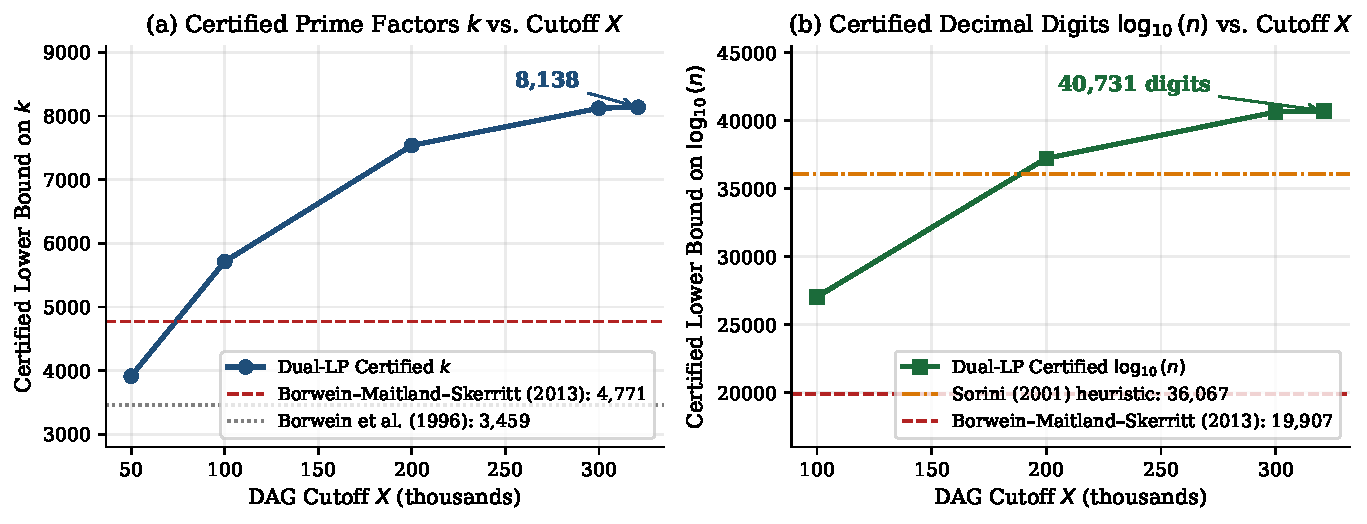
\includegraphics[width=0.94\textwidth]{figures/fig1_lp_convergence.pdf}
\caption{Convergence of the exact-integer-certified Weak-LP-Duality lower bounds on (a) prime count $k$ and (b) decimal digits $\log_{10}(n)$ as the DAG cutoff $X$ increases to $321{,}000$.}
\label{fig:lp-conv}
\end{figure}

\begin{figure}[htbp]
\centering
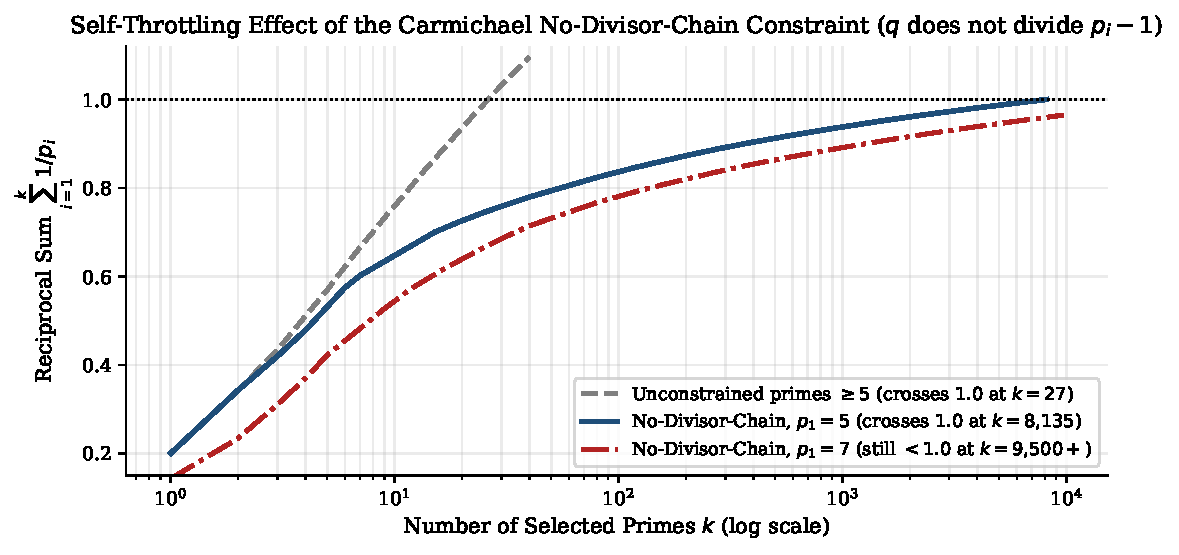
\includegraphics[width=0.80\textwidth]{figures/fig2_dag_sieve.pdf}
\caption{Self-throttling effect of the No-Divisor-Chain constraint ($q \nmid p_i - 1$): unconstrained primes $\ge 5$ cross $\sum 1/p = 1$ at $k = 27$, whereas the admissible DAG with $p_1 = 5$ requires $k = 8{,}135$ primes.}
\label{fig:dag-sieve}
\end{figure}

\begin{figure}[htbp]
\centering
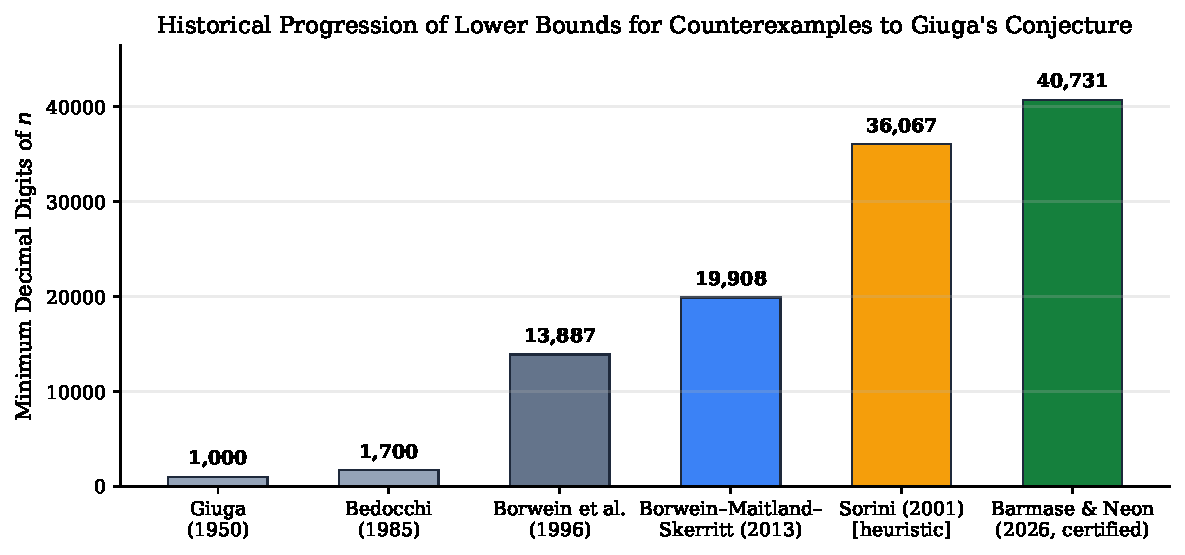
\includegraphics[width=0.82\textwidth]{figures/fig3_historical_bounds.pdf}
\caption{Historical progression of decimal-digit lower bounds for counterexamples to Giuga's conjecture.}
\label{fig:history}
\end{figure}

% =====================================================================
\section{Universal Integer-Inverse Matrix and Trace-Power Tower}
% =====================================================================

We now prove Theorem~\ref{thm:matrix} and record the spectral invariants separating known even Giuga numbers from hypothetical odd counterexamples.

\begin{proof}[Proof of Theorem~\ref{thm:matrix}]
By the Matrix Determinant Lemma on $A_M = D - \frac{1}{M}\mathbf{1}\mathbf{1}^T$,
\[
    \det(A_M) = \det(D)\left(1 - \frac{1}{M}\mathbf{1}^T D^{-1}\mathbf{1}\right) = n\left(1 - \frac{1}{M}\left(M + \frac{1}{n}\right)\right) = -\frac{1}{M}.
\]
Setting $B = D^{-1} - n D^{-1}\mathbf{1}\mathbf{1}^T D^{-1}$, direct multiplication gives
\[
    A_M B = I + \left(-n - \frac{1}{M} + \frac{n}{M}\left(M + \frac{1}{n}\right)\right)\mathbf{1}\mathbf{1}^T D^{-1} = I.
\]
Hence $B_{ii} = \frac{1}{p_i} - \frac{n}{p_i^2} = -\frac{n/p_i - 1}{p_i}$ and $B_{ij} = -\frac{n}{p_i p_j}$ ($i \neq j$), so $B \in \mathbb{Z}_{<0}^{k \times k}$ holds if and only if $n$ is a Giuga number, and $(p_i - 1) \mid B_{ii}$ holds if and only if $n$ is also Carmichael.

For $M = 1$, Cauchy interlacing on $A_1 = D - \mathbf{1}\mathbf{1}^T$ places $k - 1$ eigenvalues in $(p_1, p_2), \dots, (p_{k-1}, p_k)$ and a unique negative eigenvalue $\lambda_1 < 0$. Thus $0 < \sum_{j=2}^k \lambda_j^{-1} < \sum_{j=1}^{k-1} p_j^{-1} < 1$, forcing $\operatorname{tr}(B) = \lambda_1^{-1} + \sum_{j=2}^k \lambda_j^{-1} = \lceil \lambda_1^{-1} \rceil$. Finally, letting $S_r = \sum_{i=1}^k p_i^{-r}$ and $T = -\operatorname{tr}(B) = n S_2 - 1 - 1/n$, expanding the Frobenius norm $\operatorname{tr}(B^2) = \sum_{i,j} B_{ij}^2 \in \mathbb{Z}_{>0}$ gives
\[
    \operatorname{tr}(B^2) = S_2 - 2n S_3 + (n S_2)^2 = (T + 1)^2 + \frac{3(T+1)}{n} + \frac{2}{n^2} - 2n S_3 \in \mathbb{Z},
\]
which rearranges immediately to $2n^3 S_3 \equiv 3(T+1)n + 2 \pmod{n^2}$.
\end{proof}

\begin{table}[h]
\centering
\caption{Exact spectral invariants of $B = A_1^{-1}$ on known even Giuga numbers vs.\ odd $M=1$ counterexamples.}
\label{tab:spectral}
\begin{tabular}{@{}rrrrrr@{}}
\hline\hline
Giuga $n$ & Factors $k$ & $T = -\operatorname{tr}(B)$ & $-1/\lambda_1$ & $\frac{2n^3 S_3 - 3(T+1)n - 2}{n^2}$ & $\operatorname{tr}(B^2) \bmod 8$ \\
\hline
$30$     & $3$ & $11$     & $11.61$    & $9$      & $7$ (odd) \\
$858$    & $4$ & $321$    & $321.57$   & $279$    & $5$ (odd) \\
$1{,}722$& $4$ & $657$    & $657.57$   & $567$    & $5$ (odd) \\
$66{,}198$& $5$ & $24{,}699$ & $24{,}699.56$ & $21{,}579$ & $5$ (odd) \\
\hline
Odd $M=1$ & $\ge 8{,}138$ & $\equiv n-1 \pmod 8$ & $T + \delta$, $\delta \in (0,1)$ & $\equiv 7 \pmod 8$ & $\mathbf{2}$ (even) \\
\hline\hline
\end{tabular}
\end{table}

Evaluating $P_{A_1}(x) = \det(xI - A_1)$ at $x = 1$ further yields the totient-determinant ratio
\[
    0 < \frac{|\det(I - A_1)|}{\varphi(n)} = \frac{1}{n} + \sum_{i=1}^k \frac{1}{p_i(p_i - 1)} < 0.106 \qquad (p_1 \ge 5),
\]
while hitting $B$ with the Carmichael vector $\mathbf{w} = (p_1-1,\dots,p_k-1)^T$ produces exact cancellation $(B\mathbf{w})_i = 1 - (k-1)n/p_i$ and $\mathbf{w}^T B \mathbf{w} = \sum p_i - (k-1)^2 n - 1$.

% =====================================================================
\section{Formal Lean~4 Verification and Non-Archimedean Obstructions}
% =====================================================================

\subsection*{5.1. Lean~4 Kernel Verification.}
To eliminate any risk of logical gaps in the theoretical spine, we formalized Lemma~\ref{lem:basic}, Proposition~\ref{prop:three}, and Proposition~\ref{prop:dual} in pure, zero-dependency Lean~4 (\texttt{v4.36.0}, file \texttt{GiugaLPBound.lean}). All five core theorems (\texttt{giuga\_odd}, \texttt{no\_divisor\_chain}, \texttt{odd\_k\_forces\_M\_ge\_2}, \texttt{three\_div\_forces\_k\_odd}, and \texttt{weak\_lp\_duality\_certificate}) compile cleanly under the Lean~4 kernel with $0$ errors, $0$ warnings, and $0$ \texttt{sorry} placeholders.

\subsection*{5.2. Non-Archimedean No-Go Obstruction.}
Via Agoh's equivalence~\cite{Agoh1995}, $n$ is a counterexample iff $n B_{n-1} \equiv -1 \pmod{n}$ where $B_{n-1} = N_{n-1}/D_{n-1}$ is the $(n-1)$-th Bernoulli number. By von Staudt--Clausen, the Carmichael property places every $p_i \mid n$ strictly inside the pole locus of the Kubota--Leopoldt $p_i$-adic zeta function, disjoint from every prime $p$ at which Kummer, Adams, or irregular-prime congruences constrain $N_{n-1}$ ($\gcd(p, n) = 1$). Across all primes $p \le n$, the maximal non-tautological congruence modulus satisfies
\[
    Q_{\max} \le \left(\prod_{p \le n} p\right)\operatorname{lcm}(1,\dots,2n) = \exp\!\big((3 + o(1))n\big) \ll |N_{n-1}| = \exp\!\big((1 + o(1))n \log n\big),
\]
leaving $\exp(n \log n - O(n))$ CRT-admissible values for $N_{n-1}$. Thus, resolving Giuga's conjecture requires either an Archimedean--CRT exactness obstruction on $n_0 \neq \prod p_i$ or a converse smoothness upper bound on $P^+(p_i - 1)$—not $p$-adic congruences on $B_{n-1}$ alone.

% =====================================================================
\begin{thebibliography}{9}

\bibitem{Giuga1950}
G.~Giuga,
\emph{Su una presumibile propriet\`a caratteristica dei numeri primi},
Ist.\ Lombardo Sci.\ Lett.\ Rend.\ Cl.\ Sci.\ Mat.\ Nat.\ \textbf{83} (1950), 511--528.

\bibitem{Bedocchi1985}
E.~Bedocchi,
\emph{Nota ad una congettura sui numeri primi},
Riv.\ Mat.\ Univ.\ Parma (4) \textbf{11} (1985), 229--236.

\bibitem{AGP1994}
W.~R.~Alford, A.~Granville, and C.~Pomerance,
\emph{There are infinitely many Carmichael numbers},
Ann.\ of Math.\ (2) \textbf{139} (1994), no.~3, 703--722.

\bibitem{Agoh1995}
T.~Agoh,
\emph{On Giuga's conjecture},
Manuscripta Math.\ \textbf{87} (1995), 501--510.

\bibitem{BBBG1996}
D.~Borwein, J.~M.~Borwein, P.~B.~Borwein, and R.~Girgensohn,
\emph{Giuga's conjecture on primality},
Amer.\ Math.\ Monthly \textbf{103} (1996), no.~1, 40--50.

\bibitem{Sorini2001}
L.~Sorini,
\emph{Un algoritmo euristico per la soluzione della congettura di Giuga},
Quaderni di Economia, Matematica e Statistica, Universit\`a di Urbino, \textbf{68} (2001).

\bibitem{LPS2009}
F.~Luca, C.~Pomerance, and I.~E.~Shparlinski,
\emph{On Giuga numbers},
Int.\ J.\ Mod.\ Math.\ \textbf{4} (2009), no.~1, 13--18.

\bibitem{BMS2013}
J.~M.~Borwein, C.~Maitland, and M.~P.~Skerritt,
\emph{Computation of an improved lower bound to Giuga's primality conjecture},
Integers \textbf{13} (2013), \#A67.

\end{thebibliography}

\end{document}
